% Chapter 3

\chapter{Design} % Main chapter title

\label{Chapter3} % For referencing the chapter elsewhere, use \ref{Chapter1} 

\lhead{Chapter 3. \emph{Design}} % This is for the header on each page - perhaps a shortened title

%----------------------------------------------------------------------------------------

% \emph{How the product was designed, with discussion of design alternatives (referring to Appendix B for details).}
% 
% \emph{Diskuter de viktigste funksjonene i ditt design og hvordan det har utviklet seg, fremhev noen nye/originale funksjoner.}


This chapter will describe the system in a top-down manner. After explaining the initial design requirements, the system viewed as a whole will be described, then the large logical modules and their relationships, then their individual qualities.

\section{Design choices} % (fold)
\label{sec:design_choices}

Seen as a black box, the system consumes metadata and emits predictions.

\begin{figure}[h]
  \centering
    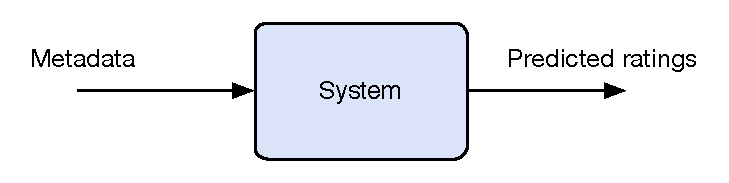
\includegraphics{Figures/dataflow}
  \caption{The system consumes metadata, and emits predicted ratings.}
  \label{fig:dataflow}
\end{figure}

The system is inherently data-driven. Every step consumes data, processes it, and emits data -- each conforming to simple interfaces in both ends.

More specifically, the system consists of three logical steps:

\begin{enumerate}
  \item Data gathering
  \item Sentiment analysis
  \item Rating prediction
\end{enumerate}

The steps sequentially process data for the next one to use, as illustrated in figure~\ref{fig:dataflow_modular}, and invoke each other through simple interfaces. In the next sections, each step will be briefly described. Implementation details are deferred to chapter~\ref{Chapter4}.

\begin{figure}[h]
  \centering
    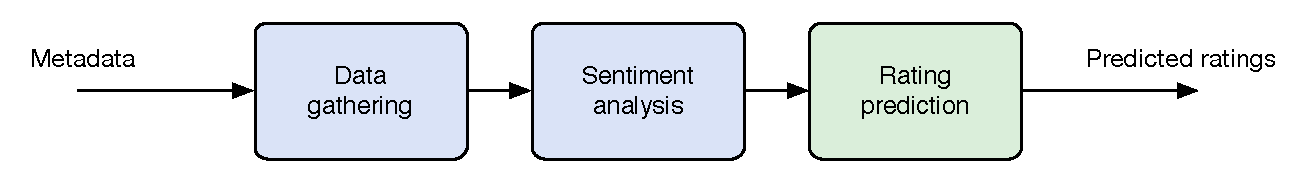
\includegraphics[width=\textwidth]{Figures/dataflow-modular}
  \caption{The high-level system design, depicted in the manner in which data flows through it.}
  \label{fig:dataflow_modular}
\end{figure}

% Although this application will only run in small scale, it is designed to be easily adaptable to fit functional models like the MapReduce programming model~\cite{Dean:2008:MSD:1327452.1327492}, and thus tackle theoretically unbounded amounts of data given the right circumstances.

Although the steps below are designed to handle \emph{sets of movies} at a time, to simplify, let us examine how they work for each single movie.

\section{Data gathering} % (fold)
\label{sec:data_gathering_step}

The data gathering step consumes movie metadata, and emits a list of Twitter messages.

It performs the following two rough steps:

\begin{enumerate}
  \item Query Twitter for relevant content based on given metadata.
  \item Extract textual messages from search results.
\end{enumerate}

As we shall see in later chapters, actually retrieving relevant content from Twitter is quite a bit harder than it should initially seem.

% section data_gathering (end)

\section{Sentiment analysis} % (fold)
\label{sec:sentiment_analysis_step}

The sentiment analysis step assigns a sentiment class to each associated Twitter message from the previous step. The messages are labeled as either ``positive'', ``neutral'', or ``negative''.

Other work~\cite{agarwal2011sentiment} has included a separate label for messages that were unreadable by the human annotator, but seeing as we're using a third-party sentiment classifier we are unable to experiment with this distinction.

% section sentiment_analysis (end)

\section{Rating prediction} % (fold)
\label{sec:rating_prediction_step}

The rating prediction step takes a list of sentiments, and emits a predicted rating value.

To turn the sentiment classes into a single rational number, two steps are taken:

\begin{enumerate}
  \item Each sentiment class is mapped to a real number value.
  \item The real values are reduced into a single prediction by averaging them.
\end{enumerate}

% section rating_prediction (end)

